\documentclass[a4paper, 11pt]{article}
\usepackage{graphicx}
\usepackage{algorithm}
\usepackage{algpseudocode}
\usepackage{amsmath}
\usepackage{tikz}

%\usepackage[a4paper,top=2cm,bottom=2cm,left=2.4cm,right=2.4cm]{geometry}

\usepackage{listings}

\title { Interactive Graphics Project\\ \bigskip \large IG Sapienza}
\date{22 September 2019}
\author{Silvio Dei Giudici 1708962 , \\Marco Morella 1693765, \\Fortunato Tocci 1708962}

\begin{document}

\maketitle

\section{USER MANUAL PART}
\section{User Manual}
%esponi cosa può fare l'utente (non specificare cosa succede internamente perchè questo lo specificherai nell'ultima sezione)
%selezione del personaggio, giorno/notte (anche in game), difficoltà, comandi

%TECHNICAL PART
\section{Development environment}
\subsection{WebGL}
%parla delle cose che stanno nelle slide eventualmente (un riassuntino), tipo vertex e fragment shader, come si rappresentano oggetti (vertici)
%come rappresentare movimenti (con matrici ecc)
\subsection{Library and tools}
%three js, OrbitControls, Browser firefox (uso della console), IDE (se vuoi)

\section{Technical Solutions}

\subsection{Hierarchical models}

\subsubsection{Animals}
We will now analyze all hierarchical models used in the project.\\
For simplicity, we will only analyze the most complex hierarchical animal model, the fox, since the other two are similar and easier.\\
This is the graph of the final model, to avoid cluttering, i've defined as Face Details all son nodes of head: both ears, both eyes and the nose, which are all brothers.\\
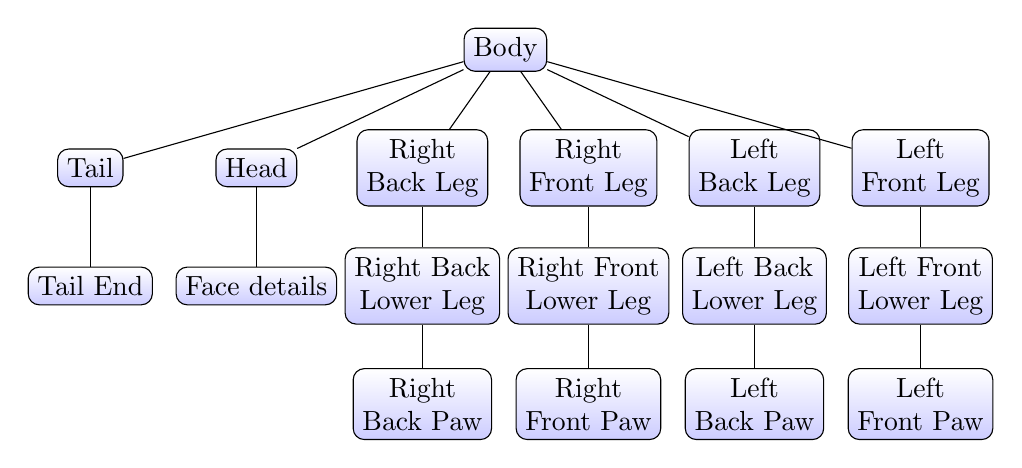
\begin{tikzpicture}[sibling distance=6em,
  every node/.style = {shape=rectangle, rounded corners,
    draw, align=center,
    top color=white, bottom color=blue!20}]]
  \node {Body}
    child { node {Tail}
      child { node {Tail End} }}
    child { node {Head}
      child { node {Face details} }}
    child { node {Right\\Back Leg}
      child { node {Right Back\\Lower Leg}
        child { node {Right\\Back Paw} } }}
    child { node {Right\\Front Leg}
      child { node {Right Front\\Lower Leg}
        child { node {Right \\Front Paw} } }}
    child { node {Left\\Back Leg}
      child { node {Left Back\\Lower Leg}
        child { node {Left\\Back Paw} } }}
    child { node {Left \\Front Leg}
      child { node {Left Front\\Lower Leg}
        child { node {Left\\Front Paw} } }};
      
\end{tikzpicture}
It is self-explanatory, every object in the second line/level is a child of Body and thus are all siblings. Each of the four upper part of the leg has a child being the lower part which has another child paw.

In the previous part i talked about "direct" if they are present in the createNode function relative to that horse's part. As an example:. 
\begin{lstlisting}
    const rightBackLegGeometry = new THREE.BoxBufferGeometry(0.2*size, 0.4*size, 0.2*size);
    this.rightBackLeg = new THREE.Mesh(rightBackLegGeometry, this.skinMaterial);
    this.rightBackLeg.position.set(-0.25*size, -0.3*size, -0.45*size);
    this.group.add(this.rightBackLeg);

    const rightBackDownLegGeometry = new THREE.BoxBufferGeometry(0.2*size, 0.4*size, 0.2*size);
    this.rightBackDownLeg = new THREE.Mesh(rightBackDownLegGeometry, this.blackMaterial);
    this.rightBackDownLeg.position.set(0, -0.4*size, 0);
    this.rightBackLeg.add(this.rightBackDownLeg);

    const rightBackPawGeometry = new THREE.BoxBufferGeometry(0.2*size, 0.1*size, 0.2*size);
    const rightBackPaw = new THREE.Mesh(rightBackPawGeometry, this.whiteMaterial);
    rightBackPaw.position.set(0, -0.25*size, 0);
    this.rightBackDownLeg.add(rightBackPaw);
\end{lstlisting}
This is the standard way in three js to create a hierarchical model. A leg has been deemed the most noteworthy example we could make. Each element has to be created as a new geometry with its measures and have the material added(which can include a texture as well as many other properties). The upper part of the leg gets added to this.group, which represent the main part of the animal(the body) and positioned w.r.t. the body. Afterwards the lower part gets created and added to the upper leg and the same happens to the paw in relation to the lower.\\
\subsection{Trees}
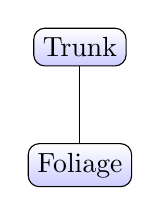
\begin{tikzpicture}[sibling distance=6em,
  every node/.style = {shape=rectangle, rounded corners,
    draw, align=center,
    top color=white, bottom color=blue!20}]]
  \node {Trunk}
    child { node {Foliage}};
\end{tikzpicture}
\\
Simply enough, we made trees in such a way that they have different heights, and they are made in such a way that an iteration occurs over the creation where foliage gets added veritcally until we reach the desired height, so each cube of foliage is a child of the trunk.
%Descrivi gli altri modelli hierarchical: macchine, terreni, tronchi sul fiume, cespugli

%ogni personaggio, auto, tree, ambiente(River, Road) (ricorda che hai track --> tree/auto (sono figli del track))
\subsection{Lights and Shadows}
%parla della luce del sole (con i dettagli della luce scelta), la luce del lampione (con alternanza giorno notte)
\subsection{Texture}
Textures are the basis of most computer graphic applications.\\
Before starting this section, we will see three kind of textures we have applied to the same object in our project: the logs floating the river.\\
\begin{figure}[!h]
\minipage{0.3\textwidth}
  \includegraphics[width=\linewidth]{sidelog.jpg}
  \caption{Standard}\label{fig:tex_img}
\endminipage\hfill
\minipage{0.3\textwidth}
  \includegraphics[width=\linewidth]{sidelognormal.jpg}
  \caption{Normal}\label{fig:n_img}
\endminipage\hfill
\minipage{0.3\textwidth}%
  \includegraphics[width=\linewidth]{sidelogao.jpg}
  \caption{AO}\label{fig:ao_img}
\endminipage
\end{figure}
\\
In our game, we used the textures to give detail to our models, obviously all images used are from free-of-use libraries and sites.\\
A normal map texture is a texture which uses rgb values to signify the orientation of the surface normal by corresponding those values to the xyz of the surface normal at any given pixel. Basically it gives a lower-detailed model(e.g. a cube) finer details with respect to the interaction with the light. In our project we've decided to add them only to two objects:
\begin{itemize}
\item Logs : in order to make the logs more realistic(and as a collateral, more "dynamic") we've added to them a normal map. But since they are made of wood, they should not reflect much light and thus we made them a MeshPhongMaterial, which is a three js material which won't shine as much as the Lambert one. While we were not using the Phong material, it was reflecting an absurd amount of light with the normal mapping active and would've been an extremely realistic effect on most other materials.
\item Foliage and Bushes : in nature, most trees' crown and most king of bushes shine under the light, we applied a normal map to capture this shininess.
\end{itemize}
And ambient occlusion(AO) texture is used to add shadow details to the object it is applied to, pronuncing its effects and giving a better sense of depth.
The decision to not apply textures to all our object was agreed by all the members because after approaching the state that can be seen in the repo, all subsequent texture implementation were making the project look worse, less sharp and more messy than it needed to be. For this reasons we didn't put any texture on the animals or the ground.\\
Also in the case of the water, we tried different combinations of Texture/Normal Texture, but the final one without any normal mapping was way better looking than any other combination and since we already had normal textures in the project it didn't seem a good idea to make it worse purposely.\\
\subsection{Animations}
Each of our animations has been hand-made by us over the hierarchical models we've implemented.\\
Since they are all quite similar, we will analyze the most complex and articulate one : the Fox.\\
\begin{center}
	\includegraphics[scale=0.22]{FoxAnimation.jpeg}\\
\end{center}
In the previous figure, the orange arrows represent the rotations(with respect to the x axis going in the opposite direction from the viewer towards the fox) which will affect the animal, namely the torso rotation upward, the upper leg and lower leg rotating in opposite direction. Furthermore the animal will traslate toward the directions it is facing, Z positives in our image, and upward in the Y axis.\\ When the Fox reaches the peak of its jump, it will suffer rotations opposed to the one we've described, in order to reset for the next jump, since it is simply the inverse of these, an image was deemed unnecessary.\\
Before doing all of this, when recognizing an input from the user, we check what key he has pressed and based on that we rotate the animal to do the correct jump.\\
As we were discussing, the Fox has the most complex animations, since we wanted a feel of simpicity for the sheep, and the chicken has inherently a simple jump. Thus the latters have parametric jumps where, by the use of trigonometric functions we apply rotations back and forth.\\
The fox is based on a counter animation. After noticing how many renders/jump functions were needed by the animal to conclude the jump animation, we divided the functions and in the first half we do the animation described in photo, while in the second part we do the exact opposite rotations to get back in place.\\
To compensate this complexity difference, the Sheep has also flapping ears which move when jumping and the Chicken flaps its wings.\\
Apart from the jump animations, all animals have two other animations:
\begin{itemize}
\item SunkAnimation: which happens whenever an animal falls in to the river. This animation shows the animal sinking(dropping hastly along the y axis) and a splash effect starts, which prompts the creation of splash particles(squares of the same color of the river, for simplicity) that rise and fall from the point of sinking.
\item CrashAnimation: happens whenever a car and the animal comes in contact. We wanted to achieve a rather humurous effect, in fact the animal gets propelled toward the air way faster than it should be, while rotating along two different directions. The details of how the detection happens will be explained in the next section.
\end{itemize}
All animations were done by using the hierarchical model of the animals and then using three js's function:
\begin{itemize}
\item : object.rotation.axis : which sets/offsets the rotation of an object along one axis  by a certain angle in radiants.
\item: object.rotateOnAxis(new Axis), which is used to rotate correctly along the original axis when the animal is rotated(and thus has its relative axis moved).
\end{itemize}
%anche l'animazione dello splash, nella sezione successiva parliamo solo della detection
%animazione degli animali, animazione auto/trunk, animazione sunk, animazione crash
\subsection{Crash, sunk and object detection}
%parla sia del crash con auto, splash del personaggio e detection dei trees/bush
\subsection{Optimizations}
%parla dell'uso dei Layers e delle animazioni che partono solo quando il personaggio si avvicina
%
%how much they increase the perfomance
%riporta la disposizione dei valori label dei livelli
In these section we are going to analyze the optimization techniques adopted in the project and how much they increase the perfomance of the game. \\

The first optimization was added using a layered organization of the random map. Indeed, at the beginning of the development we start spawning all the tracks (River or Road) in the init function and then rendering all of them (consequently also their children element) for every frame. Obviously, this may bring to some slowdowns, specially in computers without GPU. 

So, in order to resolve the issue, we simply render only the tracks that are close to the animal, in particular the tracks that are visible from the camera. 
This is done using Layer, an module provided by Three js, that allow us to label every element in the game with a value. The latter is used by the camera to know if it must render an object or not. Indeed, by default every object in the space (camera included) have value zero, as if it is a unique layer. 
Hence, in order to render a limited number of tracks $n$ in each frame, we need to assing the labels so that every track is visible for $n$ layer. The following is an example of $n=4$ that should clarify how to do it:
\begin{equation}
    \begin{array}{lllll}
	Track3: & 1 & 2 & 3 & 4\\
	Track2: & 0 & 1 & 2 & 3\\
	Track1: & 0 & 1 & 2\\
	Track0: & 0 & 1
    \end{array}
\end{equation}
if the camera is set to layer $2$ we will see tracks number $1,2,3$.
Of course in the code we find a parametric code that assign the label correctly, using the variable called $numOfLevelVisible$.
Then of course the camera need to increase its value every time the animal come near a new layer as we can see in the render function:
\begin{lstlisting}
	if(referencePositionAnimal.z > limitMax){
		actualLevelCamera++;
      	camera.layers.set(actualLevelCamera);
	}
\end{lstlisting}
here the label of the camera is increased every time the animal reach a new layer. 

The same idea is used also for cars and trunks' animations. Indeed, their movements starts only when the player is close to the track (in particular it starts only for the current, next and previous track). In order to do that we use the previous check to know if we need to update the data structure that contains all the active tracks in the game, called $actualListTracks$. Then it will used by the fuctions that animate them, scanning a fewer number of tracks. Also this optimization is adopted by the trees detection because they are child of the tracks, so they are affected by the activation of only a part of them. 
Of course if the animal try to go back there is a piece of code that decrease the camera's label and load the old tracks previously cross. \\

The final result is a more fluid game, in our tests we passed from 20 fps to 50 pfs in similar map situations. 


\section{User-game interactions}
%esponi le interazioni che l'utente può eseguire specificando cosa succede internamente (ex: ad ogni livello corrispondo 6 livelli per easy ecc)
\end{document}
